\documentclass[11pt]{article}

\usepackage[margin=0.9in]{geometry}
\usepackage{amsmath,amssymb,bm,mathtools}
\usepackage{booktabs,array,tabularx}
\usepackage{enumitem}
\usepackage{xcolor}
\usepackage{microtype}
\usepackage{listings}
\usepackage{tikz}
\usetikzlibrary{arrows.meta,positioning,shapes.geometric,calc,fit,decorations.pathreplacing}
\usepackage[hidelinks]{hyperref}

\definecolor{guideblue}{HTML}{246B9E}
\definecolor{guideorange}{HTML}{D97706}
\definecolor{guidegreen}{HTML}{2F855A}
\definecolor{guidepurple}{HTML}{7157A5}
\definecolor{guidelight}{HTML}{F4F7FA}
\definecolor{guidegray}{HTML}{4A5568}

\newcommand{\vect}[1]{\bm{#1}}
\newcommand{\dd}{\,\mathrm d}
\newcommand{\E}{\mathbb E}
\DeclareMathOperator{\Var}{Var}
\DeclareMathOperator{\Cov}{Cov}
\newcolumntype{L}[1]{>{\raggedright\arraybackslash}p{#1}}
\newcolumntype{Y}{>{\raggedright\arraybackslash}X}

\lstdefinestyle{pseudocode}{
  basicstyle=\ttfamily\small,
  keywordstyle=\color{guideblue}\bfseries,
  commentstyle=\color{guidegreen!80!black},
  numbers=left,
  numberstyle=\scriptsize\color{guidegray},
  stepnumber=1,
  numbersep=8pt,
  frame=single,
  rulecolor=\color{guideblue!45},
  backgroundcolor=\color{guidelight},
  breaklines=true,
  columns=fullflexible,
  keepspaces=true,
  showstringspaces=false,
  captionpos=b,
  morekeywords={INPUT,PRECOMPUTE,INITIALIZE,REPEAT,FOR,END,UNTIL,RETURN,solve,compare,update}
}

\tikzset{
  process/.style={rectangle,rounded corners=3pt,draw=guideblue,thick,
    fill=guideblue!7,align=center,minimum height=0.78cm,text width=3.0cm},
  data/.style={rectangle,rounded corners=3pt,draw=guidegreen,thick,
    fill=guidegreen!7,align=center,minimum height=0.78cm,text width=2.8cm},
  belief/.style={rectangle,rounded corners=3pt,draw=guidepurple,thick,
    fill=guidepurple!8,align=center,minimum height=0.85cm,text width=2.8cm},
  decision/.style={diamond,aspect=2.0,draw=guideorange,thick,
    fill=guideorange!8,align=center,inner sep=1.5pt,text width=2.3cm},
  flow/.style={-{Latex[length=2.6mm]},thick,draw=guidegray}
}

% Replace these fields.
\title{A Gentle Guide to a Scientific or Engineering Method}
\author{}
\date{\today}

\setlength{\parskip}{0.45em}
\setlength{\parindent}{0pt}

\begin{document}
\maketitle

\begin{abstract}
State the practical problem, the proposed physical or mathematical method, the quantities that are known and inferred, and what the reader will understand after finishing the guide. Keep the abstract accessible to a technically literate reader who is new to the method.
\end{abstract}

\tableofcontents

\section{The problem we want to solve}

Begin with the desired map rather than with implementation details. Let $u(\vect x,t)$ be the state, $\mu$ known physical inputs, and $q(t)$ the requested output:
\begin{equation}
 \mathcal S_\theta:\{u_0,\mu,g\}\longmapsto u(\vect x,t)
 \longmapsto q(t)=\mathcal H[u](t).
 \label{eq:desired-map}
\end{equation}
Explain why the high-fidelity solution is expensive or difficult, what the reduced or inferred model should preserve, and the regime in which predictions are intended.

\begin{center}
\fcolorbox{guideblue}{guidelight}{\parbox{0.91\linewidth}{
\textbf{Central idea.} State the one idea the reader should retain: which physics remains explicit, which quantities are learned or approximated, and why the combination is useful.
}}
\end{center}

\section{The physical or conceptual picture}

Define every state, coefficient, sign convention, coordinate orientation, and unit before presenting the complete governing equations. Use a schematic only when it makes the mechanism easier to understand.

\begin{figure}[htbp]
\centering
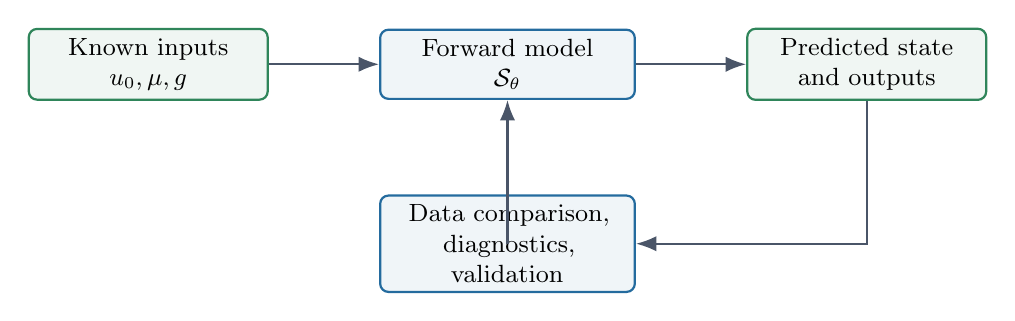
\begin{tikzpicture}[node distance=1.2cm and 1.4cm,font=\small]
  \node[data] (inputs) {Known inputs\\$u_0,\mu,g$};
  \node[process,right=of inputs] (forward) {Forward model\\$\mathcal S_\theta$};
  \node[data,right=of forward] (outputs) {Predicted state\\and outputs};
  \node[process,below=of forward] (evidence) {Data comparison,\\diagnostics, validation};
  \draw[flow] (inputs) -- (forward);
  \draw[flow] (forward) -- (outputs);
  \draw[flow] (outputs) |- (evidence);
  \draw[flow] (evidence) -| (forward);
\end{tikzpicture}
\caption{Generic relationship between inputs, the forward model, predictions, and evidence. Replace this schematic with the subject-specific mechanism when a figure is useful.}
\label{fig:concept}
\end{figure}

\section{Governing equations}

Write the forward problem in conservative form when appropriate:
\begin{align}
 \partial_t m(u)+\nabla\cdot\vect F(u,\nabla u;\mu,\theta)
 &=s(u,\vect x,t;\mu,\theta), && \vect x\in\Omega,\ t\in(0,T],
 \label{eq:governing}\\
 u(\vect x,0)&=u_0(\vect x), && \vect x\in\Omega,\label{eq:initial}\\
 \mathcal B[u]&=g, && \vect x\in\partial\Omega .\label{eq:boundary}
\end{align}

Read Eqs.~\eqref{eq:governing}--\eqref{eq:boundary} term by term:
\begin{itemize}[leftmargin=*]
 \item $m(u)$ is the stored extensive quantity or mass density;
 \item $\vect F$ is the signed conservative flux;
 \item $s$ contains physical sources, sinks, or balanced internal transfer;
 \item $\theta$ contains explicitly declared closure or inferred coefficients;
 \item $u_0$ and $g$ complete the forward problem.
\end{itemize}

State which relations are exact identities and which are constitutive assumptions. If a closure is introduced, define a residual that can be measured from high-fidelity data.

\subsection{Conservation and invariants}

For a closed system, integrate Eq.~\eqref{eq:governing} over $\Omega$:
\begin{equation}
 \frac{\dd}{\dd t}\int_\Omega m(u)\dd\vect x
 =-\int_{\partial\Omega}\vect n\cdot\vect F\dd S
 +\int_\Omega s\dd\vect x .
 \label{eq:global-balance}
\end{equation}
Use Eq.~\eqref{eq:global-balance} to specify mass, boundary-flux, uniform-state, positivity, or energy tests before calibration.

\section{What is known and what must be learned}

\begin{center}
\begin{tabularx}{0.94\textwidth}{>{\bfseries\raggedright\arraybackslash}p{0.22\textwidth}Y}
\toprule
Category & Contents \\
\midrule
Known inputs & Geometry, initial and boundary data, forcing, measured physical coefficients, and numerical conventions. \\
Unknown model terms & Closure fields, constitutive parameters, reduced operators, or discrepancy terms. \\
Observations & State samples, integrated outputs, fluxes, moments, and their sampling/processing metadata. \\
Required predictions & New initial conditions, held-out parameter cases, long rollouts, and uncertainty if requested. \\
\bottomrule
\end{tabularx}
\end{center}

If observations are collected in $\vect y$, write the observation model explicitly:
\begin{equation}
 \vect y=\mathcal H\mathcal S_\theta(u_0,\mu,g)+\vect\varepsilon,
 \qquad \vect\varepsilon\sim\mathcal N(\vect0,\vect\Sigma).
 \label{eq:observation}
\end{equation}
Explain what $\vect\Sigma$ represents. Correlated numerical or model discrepancy should not be mislabeled as independent measurement noise.

\section{Calibration before specialized probability language}

Describe the deterministic loop first: propose coefficients, solve the forward problem, compare predictions with observations, and update. Figure~\ref{fig:calibration} provides a reusable layout.

\begin{figure}[htbp]
\centering
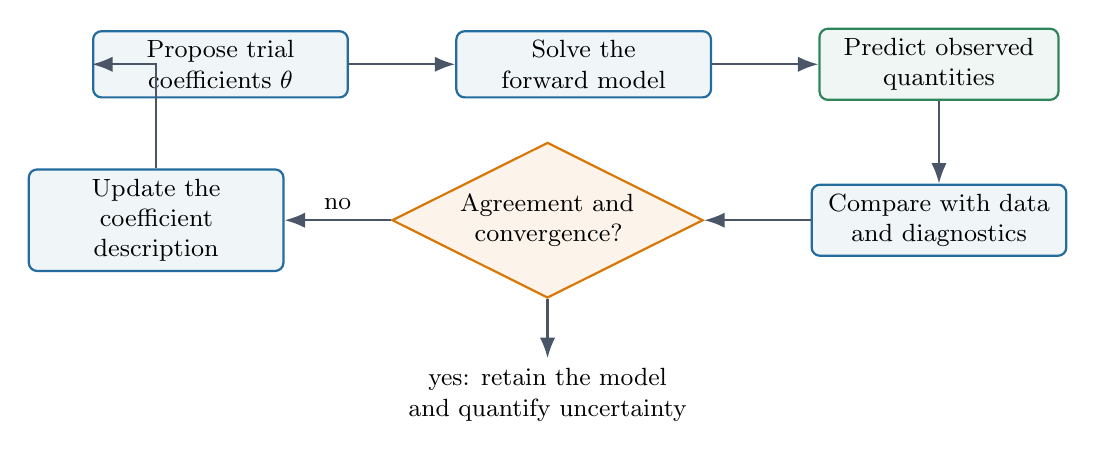
\begin{tikzpicture}[node distance=1.05cm and 1.35cm,font=\small]
  \node[process] (trial) {Propose trial\\coefficients $\theta$};
  \node[process,right=of trial] (solve) {Solve the\\forward model};
  \node[data,right=of solve] (predict) {Predict observed\\quantities};
  \node[process,below=of predict] (compare) {Compare with data\\and diagnostics};
  \node[decision,left=of compare] (stop) {Agreement and\\convergence?};
  \node[process,left=of stop] (update) {Update the coefficient\\description};
  \draw[flow] (trial) -- (solve);
  \draw[flow] (solve) -- (predict);
  \draw[flow] (predict) -- (compare);
  \draw[flow] (compare) -- (stop);
  \draw[flow] (stop) -- node[above] {no} (update);
  \draw[flow] (update) |- (trial);
  \draw[flow] (stop.south) -- ++(0,-0.75) node[below,align=center] {yes: retain the model\\and quantify uncertainty};
\end{tikzpicture}
\caption{Generic calibration and verification loop.}
\label{fig:calibration}
\end{figure}

\section{Inference or optimization formulation}

For a Bayesian formulation, separate prior, likelihood, and posterior:
\begin{align}
 \theta&\sim p(\theta),\\
 p(\vect y\mid\theta)&\propto
 \exp\!\left[-\tfrac12
 \|\vect y-\mathcal H\mathcal S_\theta\|_{\vect\Sigma^{-1}}^2\right],\\
 p(\theta\mid\vect y)&\propto p(\vect y\mid\theta)p(\theta).
 \label{eq:posterior}
\end{align}
Define the norm, covariance, parameter representation, positivity transformation, and reference scales. Explain what the posterior uncertainty includes and what structural uncertainty remains outside the assumed model.

For deterministic fitting, state the complete regularized objective instead:
\begin{equation}
 \theta_{\mathrm{MAP}}
 =\arg\min_\theta
 \frac12\|\vect y-\mathcal H\mathcal S_\theta\|_{\vect\Sigma^{-1}}^2
 +\frac12\|\theta-\theta_0\|_{\vect K^{-1}}^2 .
 \label{eq:map}
\end{equation}

\section{Numerical implementation}

Separate the state grid, coefficient representation, observation locations, and optimization variables. Describe the solver, discretization, sensitivities or adjoint, stopping criteria, and computational batching without discarding trustworthy data.

\begin{lstlisting}[style=pseudocode,caption={Generic verified calibration workflow.},label={alg:workflow}]
INPUT:
  model inputs, initial and boundary conditions
  observations and uncertainty/discrepancy model

PRECOMPUTE:
  geometry, operators, parameter basis, and observation map

INITIALIZE:
  choose a defensible parameter state theta

REPEAT:
  solve the forward model for every training case
  compare predictions with observations and invariants
  update theta using verified sensitivities or gradients
UNTIL objective, gradient, and parameter changes are small

RETURN:
  fitted model, residual diagnostics, uncertainty, validation results
\end{lstlisting}

\section{Identifiability, uncertainty, and limitations}

Explain which parameters can compensate for each other, which observations separate their effects, and which predictions leave the training distribution. Adding parameter resolution does not create information absent from the data.

Use a callout for the most consequential limitation:
\begin{center}
\fcolorbox{guideorange}{guideorange!6}{\parbox{0.91\linewidth}{
\textbf{Important limitation.} State the main structural, numerical, or data limitation and the experiment or diagnostic that can resolve it.
}}
\end{center}

\section{Validation and what counts as success}

Split by complete physical cases rather than by nearby snapshots. Report field or state error, conserved quantities, moments, fluxes, uncertainty coverage, stability, and computational cost. The decisive test is an uninterrupted rollout initialized only at the declared start or handoff time.

\begin{enumerate}[leftmargin=*]
 \item Fit or construct the model using complete training cases.
 \item Predict a held-out case without using its later states.
 \item Repeat across the available independent cases.
 \item Compare with the required simpler baseline and report failure regimes.
\end{enumerate}

\section{Recommended implementation sequence}

\begin{enumerate}[leftmargin=*]
 \item Verify inputs, units, coordinate frame, initial/boundary data, and numerical truth.
 \item Implement the forward model with known coefficients and test invariants.
 \item Fit the smallest identifiable parameterization.
 \item Diagnose residuals before adding spatial, nonlinear, nonlocal, or learned complexity.
 \item Quantify uncertainty and validate complete held-out cases and full rollouts.
\end{enumerate}

\section{Glossary}

\begin{center}
\begin{tabularx}{0.94\textwidth}{L{0.25\textwidth}Y}
\toprule
Term & Meaning in this note \\
\midrule
Forward problem & Predict the state and outputs when inputs and coefficients are specified. \\
Inverse problem & Infer unknown coefficients or inputs from observed outputs. \\
Closure & A modeled relation replacing unresolved information in a reduced description. \\
Identifiability & Ability of the available observations to distinguish parameter effects. \\
Validation & Prediction of complete cases not used to construct or calibrate the model. \\
Posterior predictive & Prediction after propagating posterior parameter uncertainty through the forward model. \\
\bottomrule
\end{tabularx}
\end{center}

\appendix
\section{Optional numerical details}

Move discretization derivations, weak forms, variable mappings, software notation, or extended checks here when they would interrupt the main explanation. Keep the main document readable without requiring the appendix.

\section{The main idea to retain}

Close with one short synthesis: what mechanism predicts the state, which uncertainty or closure is learned, what evidence supports it, and what remains to be tested.

\end{document}
